\section{EM Field Theories}

EM field theories of consciousness, notably developed in foundational work \cite{McFadden2002, McFadden2020}, suggest that consciousness emerges from the electromagnetic fields generated by neural activity rather than from the computational properties of neurons themselves. This approach shares important common ground with ECC's emphasis on physical fields and energy dynamics, though ECC takes a broader view that includes multiple forms of energetic coherence.

McFadden's consciousness electromagnetic information (cemi) field theory suggests that consciousness arises from the spatial integration of information in the brain's electromagnetic field \cite{McFadden2002}. This spatial integration provides a potential solution to the binding problem—how different aspects of conscious experience are unified into a coherent whole. Where traditional computational approaches struggle to explain this unity, EM field theories offer a natural mechanism through field coherence.

Empirical support for the importance of electromagnetic fields in neural function has grown substantially through research on ephaptic coupling \cite{Radman2007}. This work demonstrates how neurons can influence each other through local electric fields without synaptic transmission, suggesting that the brain's EM fields are not merely epiphenomenal but play an active role in neural communication and synchronization \cite{Frohlich2010}.

The relationship between EM field theories and consciousness can be understood through two distinct but complementary approaches: computational EM theories and topological EM theories \cite{Pockett2012}. Computational approaches treat the brain's electromagnetic field as a medium for information processing, while topological approaches emphasize the spatial organization and structural properties of electromagnetic fields rather than their computational capabilities.

Recent theoretical developments have suggested that field effects play crucial functional roles in neural processing \cite{Weiss2010}. These effects extend beyond simple background influence to actively shape neural computation and communication. The evidence for such field effects provides important empirical grounding for both EM field theories and ECC's broader emphasis on energetic coherence.

The binding problem, a central challenge in consciousness studies \cite{Singer2001}, takes on new significance when viewed through the lens of field theories. Rather than requiring computational mechanisms to bind different aspects of experience together, field theories suggest that binding emerges naturally from the unified nature of electromagnetic fields. This aligns with ECC's emphasis on how coherent energy states achieve integration through physical rather than computational mechanisms.

Electromagnetic approaches to consciousness also provide insight into the global integration of information in neural systems \cite{John2001}. The brain's EM fields might serve as a physical medium for information integration, creating a unified field of conscious experience without requiring additional binding or integration mechanisms. This perspective aligns with ECC's emphasis on field-like properties in conscious processing while suggesting specific physical mechanisms for their implementation.

\begin{figure}[h]
    \centering
    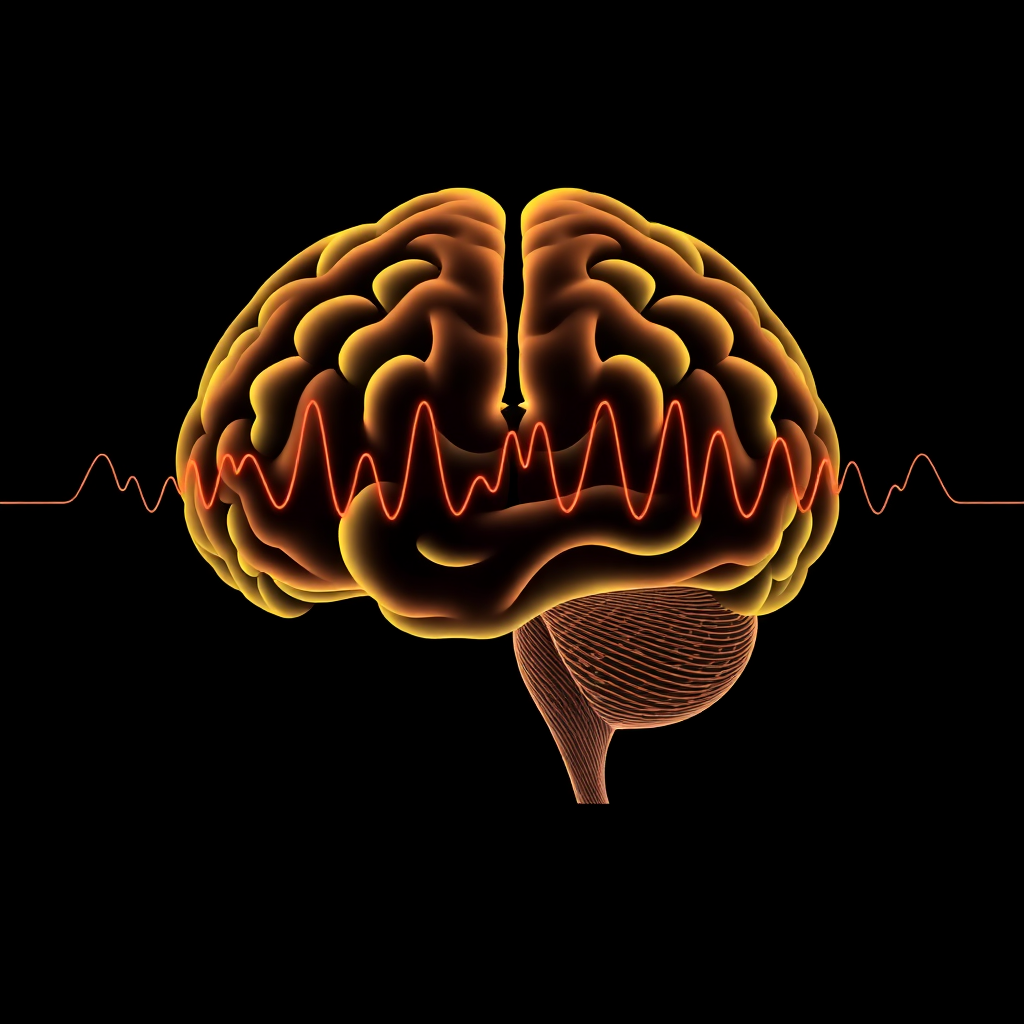
\includegraphics[width=0.8\textwidth]{images/brain_waves.png}

    \caption{Brain wave dynamics are essential for local conscious unification.}
\end{figure}

The role of electromagnetic fields in establishing and maintaining neural coherence finds substantial empirical support through recent neurobiological research \cite{Frohlich2010}. Studies have demonstrated how endogenous electric fields can guide neocortical network activity, suggesting that field effects play a crucial role in coordinating neural function. These findings provide important validation for both EM field theories and ECC's broader framework of energetic coherence.

The precise timing requirements of conscious processing raise important questions about mechanisms of neural synchronization \cite{Radman2007}. EM field theories suggest that electromagnetic fields provide a natural substrate for coordinating neural activity across different brain regions. This aligns with ECC's emphasis on how coherent energy states achieve temporal integration through physical rather than computational mechanisms.

Recent theoretical work has explored how information might be integrated in the brain's electromagnetic field \cite{McFadden2020}. While traditional approaches focus on synaptic connectivity, field theories suggest that EM fields provide an additional layer of integration that helps create unified conscious experience. This perspective complements ECC's broader framework of energetic coherence while suggesting specific mechanisms for its implementation.

The relationship between field effects and neural computation \cite{Weiss2010} reveals important questions about how physical and computational processes interact in conscious systems. Rather than treating computation and field effects as separate phenomena, EM field theories suggest they are intimately connected through the brain's electromagnetic dynamics. This aligns with ECC's view that conscious processing emerges from physical rather than purely computational mechanisms.

Experimental evidence has demonstrated how electric fields can amplify and coordinate neural activity \cite{Radman2007}. These findings suggest that field effects play a more fundamental role in neural processing than previously recognized. The ability of electromagnetic fields to influence spike timing and neural excitability provides crucial support for theories that emphasize the importance of field effects in consciousness.

The binding problem in consciousness studies \cite{Singer2001} finds potential resolution through field-based approaches. Rather than requiring computational mechanisms to bind different aspects of experience together, electromagnetic fields provide a natural substrate for integration. This aligns with ECC's emphasis on how coherent energy states achieve unity through physical rather than computational processes.

Recent developments in field theory approaches have emphasized how electromagnetic fields might contribute to both local and global aspects of conscious processing \cite{John2001}. The ability of fields to influence neural activity across multiple scales suggests they play a crucial role in creating the integrated yet differentiated character of conscious experience.

The question of how electromagnetic fields contribute to neural information processing remains an active area of investigation \cite{Barrett2011}. While some researchers emphasize the computational aspects of field effects, others focus on their role in coordinating and integrating neural activity. ECC suggests these perspectives might be unified by understanding how coherent energy states naturally support both information processing and integration through their physical dynamics.

Recent theoretical work has explored how electromagnetic fields might contribute to consciousness through their influence on neural timing and synchronization \cite{Pockett2012}. The ability of fields to coordinate activity across different neural populations suggests they play a crucial role in creating the temporal coherence characteristic of conscious experience. This aligns with ECC's emphasis on how physical mechanisms support conscious integration.

The relationship between attention and electromagnetic field effects \cite{Prinz2012} reveals important questions about conscious control mechanisms. While traditional approaches focus on synaptic mechanisms of attention, field theories suggest that electromagnetic fields might provide an additional layer of control over neural processing. This perspective complements ECC's broader framework while suggesting specific mechanisms for attentional modulation.

Empirical studies have demonstrated how electromagnetic fields shape morphogenesis and consciousness through environmental orchestration \cite{Rouleau2014}. These findings suggest that field effects play a fundamental role in both the development and ongoing function of conscious systems. This provides important support for theories that emphasize the importance of field effects in biological organization.

The integration of electromagnetic approaches with broader theories of consciousness \cite{McFadden2020} suggests productive new directions for research. By examining how field effects contribute to conscious processing while maintaining connection to other physical mechanisms, we may develop more sophisticated understanding of how consciousness emerges from biological systems.

These theoretical syntheses reveal important connections between electromagnetic field theories and other approaches to consciousness \cite{John2001}. While EM field theories provide crucial insights about specific physical mechanisms, ECC suggests these mechanisms operate within a broader framework of energetic coherence. This integration offers promising directions for future research into the physical basis of consciousness.

The future development of field-based approaches to consciousness will likely require sophisticated integration of theoretical insights with empirical investigation \cite{Singer2001}. By examining how electromagnetic fields contribute to conscious processing while maintaining connection to other physical mechanisms, we may develop increasingly sophisticated understanding of how consciousness emerges from biological systems.

In support of the EM Field view, recent research has significantly advanced our understanding of ephaptic coupling's role in neural information processing and potential contributions to consciousness. Evidence suggests that electric fields generated by neural activity can directly influence nearby neurons through non-synaptic mechanisms, creating a form of neural communication that operates alongside traditional synaptic transmission \cite{Pinotsis2023Ephaptic}. These field effects may contribute to the formation and stabilization of memory networks, suggesting a broader role for electromagnetic fields in neural information processing than previously recognized.

The concept of cytoelectric coupling has emerged as particularly significant, describing how electric fields can sculpt neural activity patterns and effectively "tune" the brain's infrastructure \cite{Pinotsis2023Cytoelectric}. Detailed modeling work has demonstrated that these ephaptic effects operate at the mesoscopic scale in human brain tissue, potentially contributing to neural synchronization and information integration \cite{Reimann2020Modeling}. Recent theoretical analysis suggests that ephaptic coupling may fundamentally contribute to brain complexity \cite{Cunha2024Ephapticity}, while studies of coincidence detector neurons in the auditory brainstem have revealed how endogenous electric fields can influence neural timing and synchronization \cite{Goldwyn2016Neuronal}. These findings align with ECC's emphasis on field effects in conscious processing, suggesting that ephaptic coupling might represent one mechanism through which the brain maintains the coherent energy states necessary for consciousness.

The role of ephaptic coupling in neural information processing suggests intriguing possibilities for how electromagnetic fields contribute to conscious experience. Beyond merely serving as a byproduct of neural activity, these fields may actively shape neural dynamics across multiple spatial scales. The ability of electric fields to modify neural timing and synchronization through ephaptic effects \cite{Goldwyn2016Neuronal} could provide a physical mechanism for the kind of rapid information integration that consciousness requires.

Research into memory network formation through ephaptic coupling \cite{Pinotsis2023Ephaptic} reveals how field effects might contribute to the stability of conscious states while allowing for dynamic reorganization. The concept of cytoelectric coupling \cite{Pinotsis2023Cytoelectric} suggests that electromagnetic fields play an active role in shaping neural architecture, potentially creating the conditions necessary for conscious processing through continuous field-mediated feedback between neurons and their environment.

Detailed modeling of mesoscopic ephaptic coupling in human brain tissue \cite{Reimann2020Modeling} has demonstrated that these effects operate at scales relevant for conscious integration. The contribution of ephaptic coupling to brain complexity \cite{Cunha2024Ephapticity} aligns with ECC's emphasis on consciousness requiring sophisticated patterns of energetic coherence. These findings suggest that ephaptic coupling might represent a crucial mechanism through which the brain achieves the field coherence necessary for conscious experience while maintaining the flexibility required for adaptive behavior.

This research indicates that electromagnetic fields in neural tissue serve not merely as epiphenomena but as active participants in neural information processing and conscious integration. The ability of ephaptic coupling to influence neural timing and synchronization without direct synaptic contact provides a potential physical basis for the kind of field-mediated integration that consciousness appears to require. These insights strengthen ECC's emphasis on field effects while suggesting specific mechanisms through which these fields might contribute to conscious experience.